% Compiler ce document 

% package de base
\documentclass[10pt,a4paper]{article}
\usepackage[utf8]{inputenc}
\usepackage{listings}

% langues
\usepackage[usenames,dvipsnames]{xcolor}
\usepackage[francais]{babel}
\usepackage[T1]{fontenc}
\usepackage{amsmath}
\usepackage{amsfonts}
\usepackage{amssymb}
\usepackage{graphicx}
\usepackage{tabularx}
\usepackage{colortbl}
\usepackage[hidelinks]{hyperref} % liens
\usepackage{fancyhdr} % En tetes / bas de page
\usepackage{helvet} % police helvetica
\usepackage[hidelinks]{hyperref}
\usepackage{xcolor} % Style pour affichage du C
\usepackage{courier} % police pour les listings

% Page de Garde -- Necessite d'installer le package titling, si probleme
% commenter la ligne suivante ainsi que les infos necessaires a la page
% de garde
\usepackage{pageGarde/HEIG_STY}

% commande pour faire des sections sans nombre 
% tout en la rajoutant dans la table des matières
\newcommand\sectionWithoutNumber[1]{\section*{#1} \addcontentsline{toc}{section}{\protect\numberline{}#1}}
\newcommand\subsectionWithoutNumber[1]{\subsection*{#1} \addcontentsline{toc}{subsection}{\protect\numberline{}#1}}
\newcommand\subsubsectionWithoutNumber[1]{\subsection*{#1} \addcontentsline{toc}{subsubsection}{\protect\numberline{}#1}}
% définition de nouvelles couleurs
\definecolor{lightblue}{rgb}{0.8,0.8,0.9}
\definecolor{grossblue}{rgb}{0,0,0.7}
%marge des pages
\setlength{\textwidth}{16cm}
\setlength{\textheight}{24cm}
\setlength{\oddsidemargin}{0cm}
\setlength{\voffset}{-1.5cm}
\setlength{\headheight}{15pt}

% set la police en arial
%% Sans-serif Arial-like fonts
\renewcommand{\rmdefault}{phv} 
\renewcommand{\sfdefault}{phv} 
\usepackage{tabularx}
\usepackage{graphicx}
\usepackage{eurosym}
\usepackage{xspace}
\newcommand{\projectname}[0]{LTANR\xspace} 

% configuration pour des listings
\lstset{ 
  showspaces=false,      
  showstringspaces=false, 
  showtabs=false,               
  tabsize=3,                     
  numbers=left
}

%enlève indentation en début de paragraphe
\setlength\parindent{0pt}

%style de l'en-tête de page
\pagestyle{fancy}

% style pour code en c
\lstdefinestyle{customc}{
  belowcaptionskip=1\baselineskip,
  breaklines=true,
  frame=L,
  xleftmargin=\parindent,
  language=C,
  showstringspaces=false,
  basicstyle=\scriptsize\ttfamily,
  keywordstyle=\bfseries\color{green!40!black},
  commentstyle=\itshape\color{purple!40!black},
  identifierstyle=\color{blue},
  stringstyle=\color{orange},
}

\lstset{escapechar=@,style=customc}
\lstset{inputencoding=utf8/latin1} %affiche les accents dans le listing

% Mise en forme de la page de titre
\author{Domingues Pedrosa João Miguel \\ Nicolas Kobel}
\title{Journal du commande de déplacement d'un chariot 
\\Laboratoire MSS complexe}

% Informations necessaires a la page de garde
% Commenter si probleme de compilation
\acro{CSN}
\cours{Conception de système numérique}
\date{\today}
\prof{Professeur: M. Messerli Etienne}

%en-tête
\lhead{Domingues João // Nicolas Kobel}
\chead{Laboratoire MSS complexe}
\rhead{\theAcro}

%pied-de-page
\lfoot{HEIG-VD}
\cfoot{\today}
\rfoot{\thepage}

\begin{document}
\maketitle
\newpage
\tableofcontents
\newpage

%Ici commence réelement l'écriture du rapport
\section{Mandat}
Le but de se laboratoire est de commandé la rotation d'un moteur. Il y a deux modes. Le mode manuel qui fait tourné le moteur temps que l'on reste appuyer sur le bouton start et le mode automatique où l'on avance du nombre de position définit. Il sera possible de modifier la vitesse de rotation

Schéma des entrée:\\
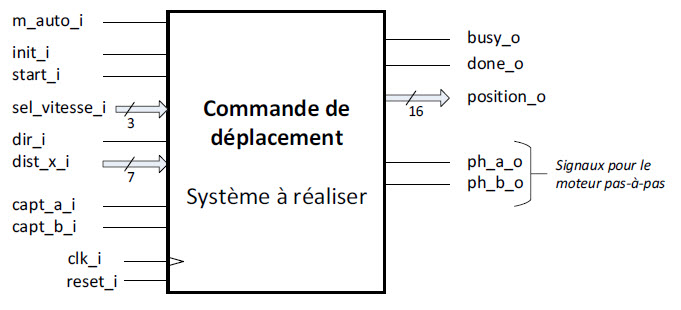
\includegraphics[scale=0.5]{images/schema_entree.jpg}

Tableau des entrées/sorties:\\
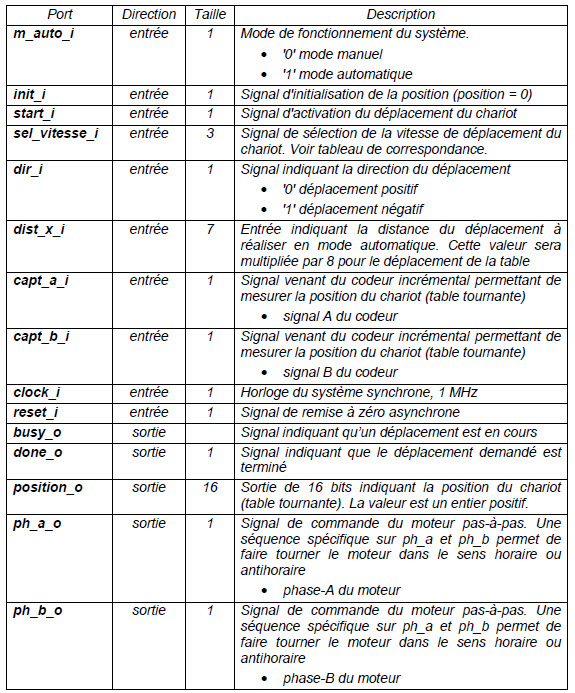
\includegraphics[scale=0.5]{images/tableau.jpg}

Tableau des vitesses:\\
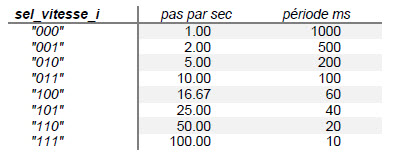
\includegraphics[scale=0.5]{images/vitesse.jpg}

Chronogramme pour commander le moteur:\\
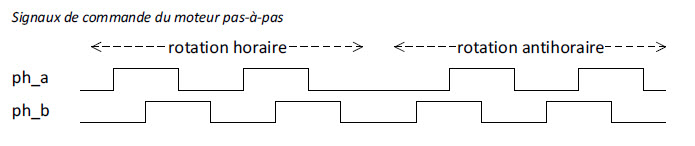
\includegraphics[scale=0.5]{images/cmd_moteur.jpg}
\newpage
\section{Analyse}
\subsection{Commande des moteurs}
Pour la commande des moteurs, nous avons fait la séparation suivante. La vitesse correspond à un diviseur d'horloge qui dépendra de la valeur de celui-c. Pour le parcours de distance en mode automatique, il s'agit que d'un compteur dont on charge la valeur définit au début du cycle et qui va décrémenter à chaque pas. Les pas sont dépendant de la vitesse, il faudra donc utilisé la sortie du diviseur d'horloge pour avoir la référence. Il génére une pulse lorsque l'on arrive à la fin de la distance.

La génération de commande se fait via une MSS. Elle reçoit en entrée le signal \texttt{start}, la direction, le mode (manuel/auto), la fin de distance pour le mode automatique et le diviseur d'horloge pour la vitesse. Il indique en  sortie si le moteur est occupé ou non et fait les différent changement de phase pour le moteur. Il s'occupe donc de faire les cycle moteur comme indiqué sur le chronnogramme lorsque celui si est en marche.

L'acquisition de position a été repris de l'ancien laboratoire de Domingues Pedrosa João Miguel.
\subsubsection{Organigramme}
Il faut faire attention au lorsque l'on avance d'un pas, il faut faire attention d'attendre sur le diviseur de fréquence afin que l'on est bien la bonne vitesse pour la rotation du moteurs.\\
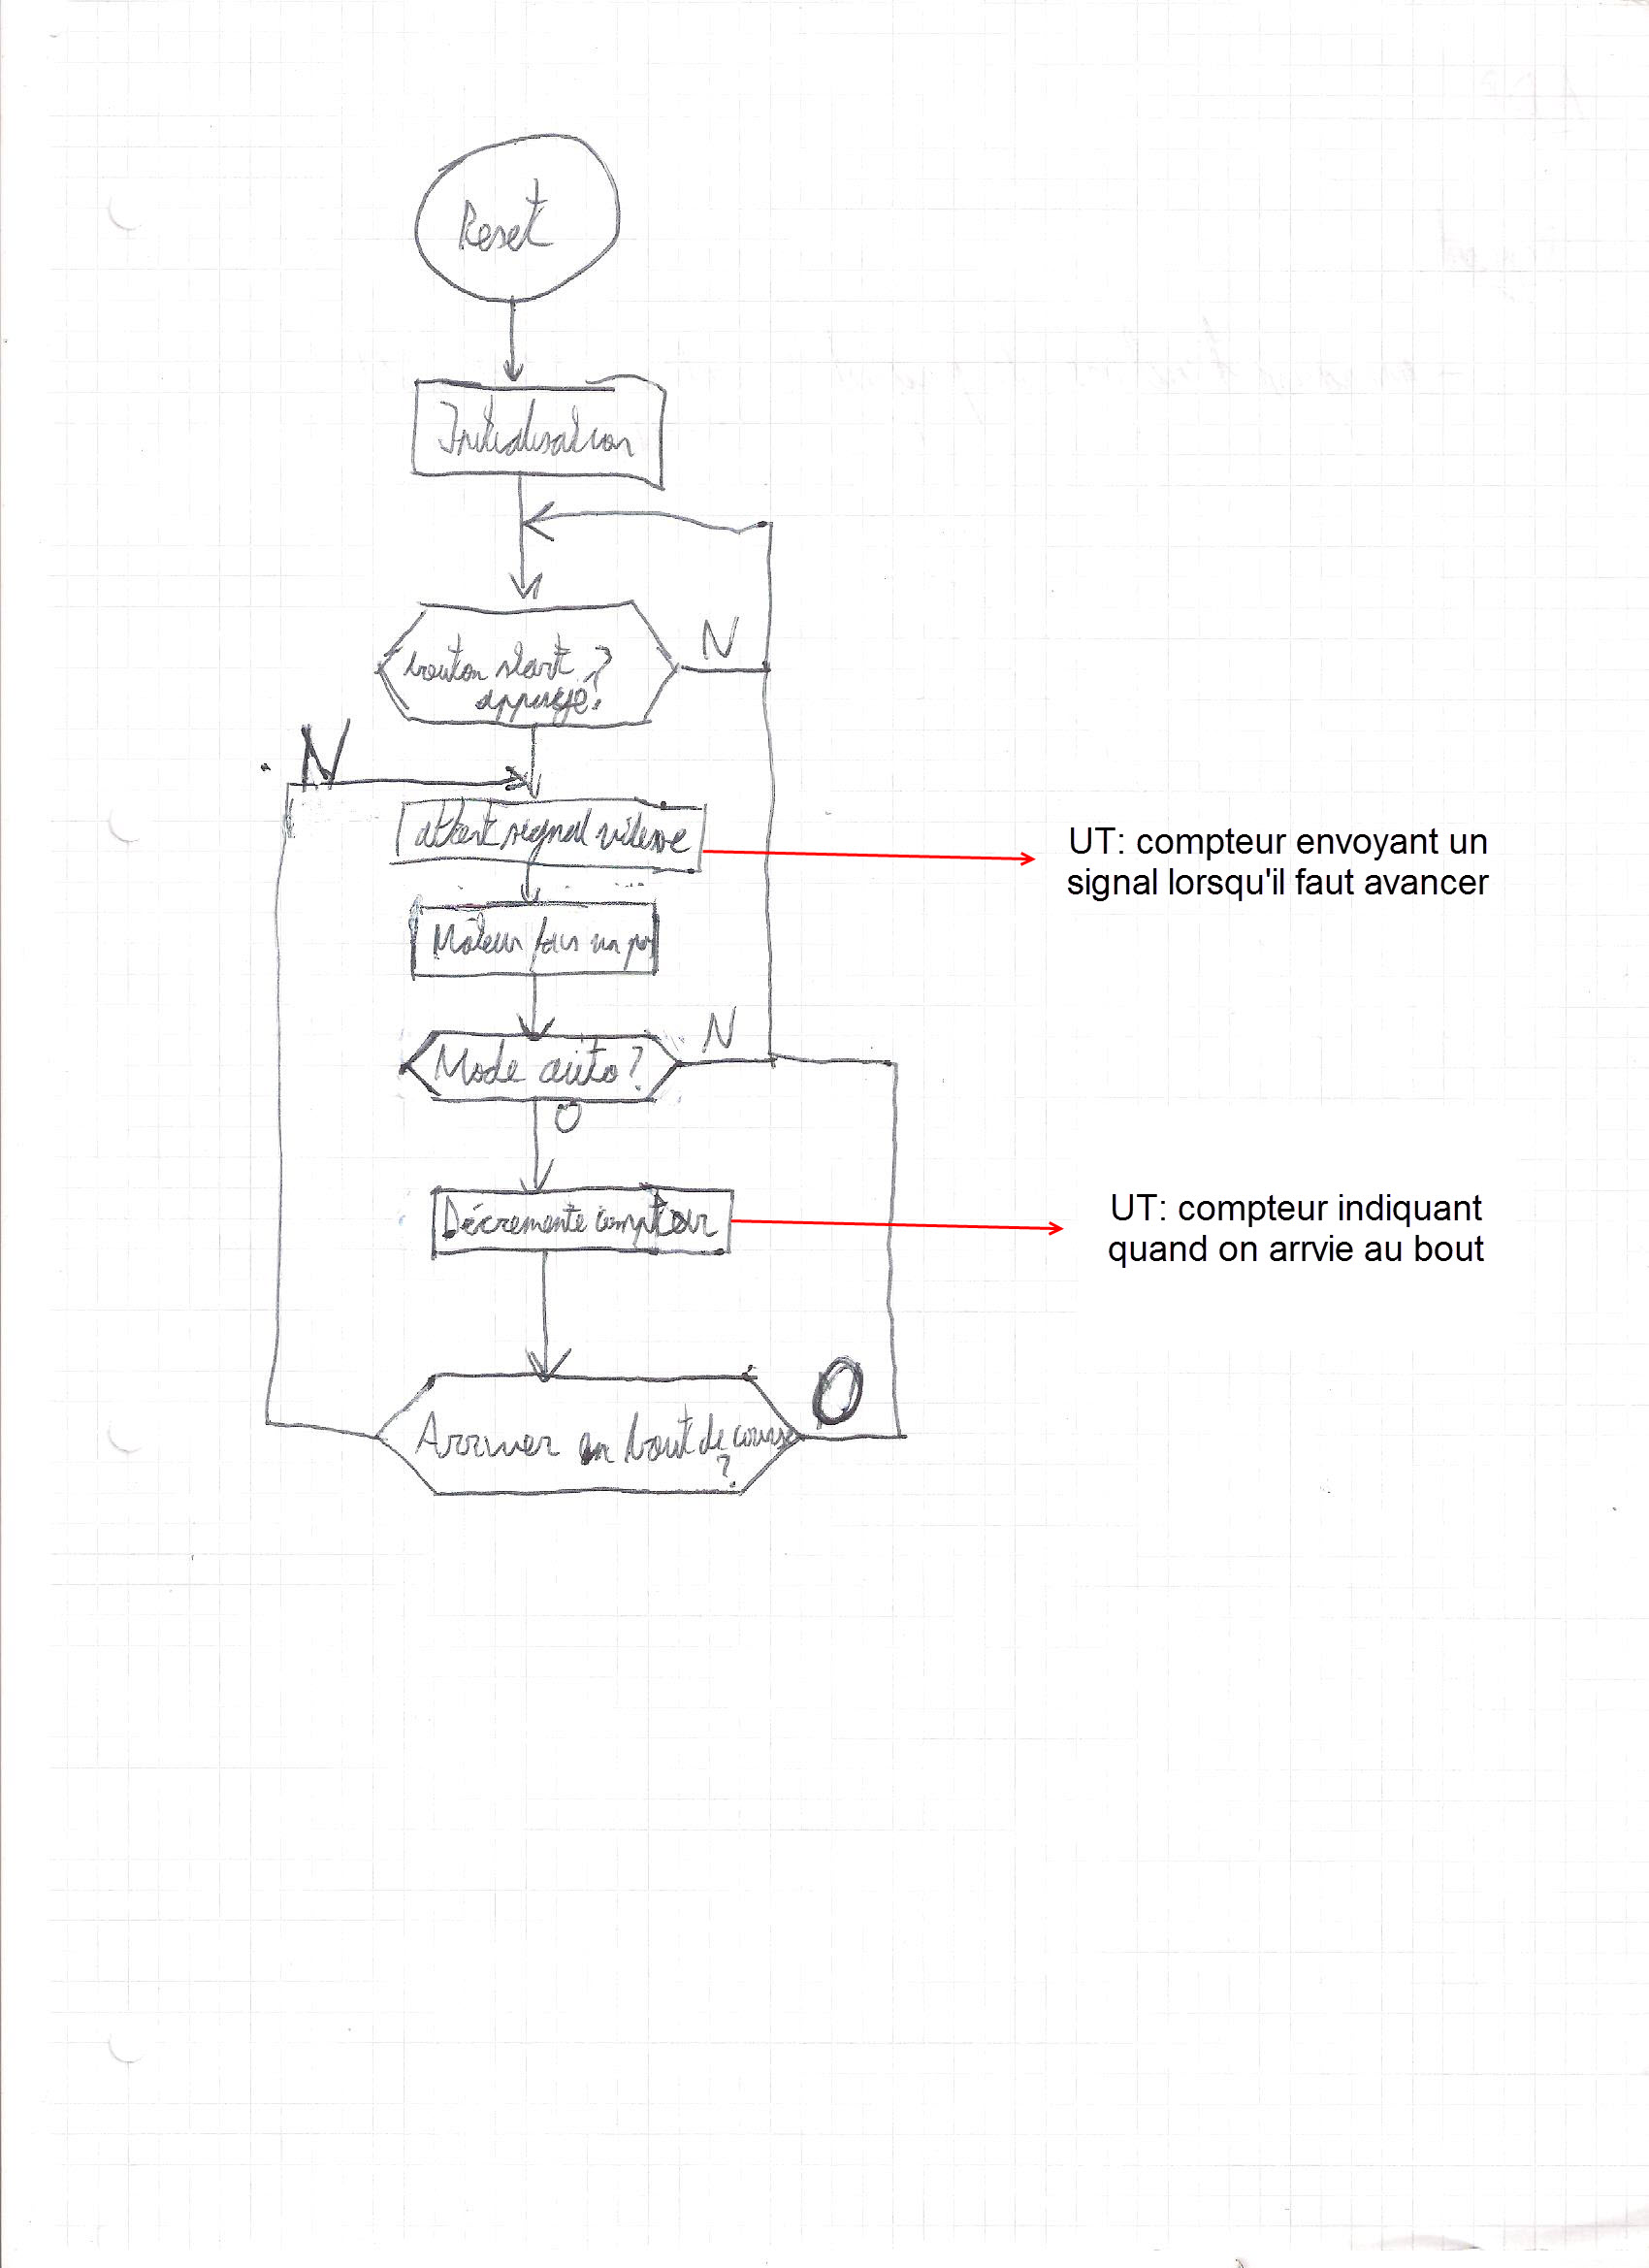
\includegraphics[scale=0.5]{images/orga.jpg}

\subsubsection{MSS génération de commande}
\includegraphics[scale=0.5]{images/MSS.jpg}

\newpage
\section{Schéma}

\newpage
\section{Simulation}
Pour les tests, nous avons testé que le fonctionnement normal dans les deux modes. En mode manuel, nous avons fait forcer le \texttt{div\_clk} à un afin de voir lorsque l'on appuie sur \texttt{start} les sortie \texttt{ph\_a} et \texttt{ph\_b} changeait et exécutait la bonne séquence. Le mode automatique, nous avons vérifier qu'après un flanc du \texttt{start} les sorties changer le bon nombre de fois. Durant c'est deux tests, nous avons aussi vérifier que les sorties \texttt{busy} et \texttt{done} correspondant au état attendu durant que le moteur fonctionne ou est à l'arrêt. Par manque de temps des tests plus poussé n'ont pas pu être effectuer.Par exemple, nous n'avons pas pus tester l'initialisation avec l'entrée \texttt{init} ou les deux sens de rotation, ici nous avons tester quand sens anti-horaire.\\

Durant les tests, nous nous somme aperçu de deux erreurs d'implémentation. La première est que lorsque l'on est en mode automatique, il faut laisser le bouton \texttt{start} appuyer jusqu'au prochain signal du \texttt{clk\_div}. Cela peut durer jusqu'à une seconde selon la vitesse sélectionner.La deuxième est que l'on fait un pas de plus que le nombre définit en mode automatique. Par manque de temps, nous n'avons pas pu les corriger.

\begin{tabular}{ll}

Chronogramme (Mode Manuel): & Chronogramme (Mode Auto):\\\\
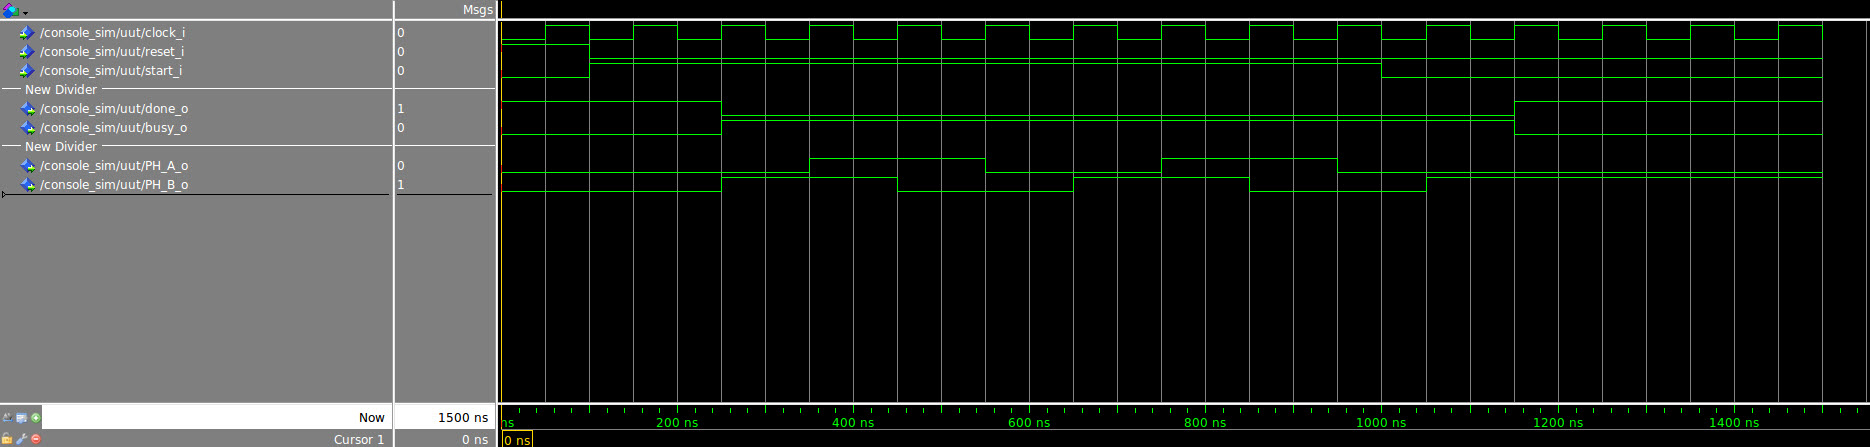
\includegraphics[angle=90,scale=0.45]{images/manualSim.jpg} & 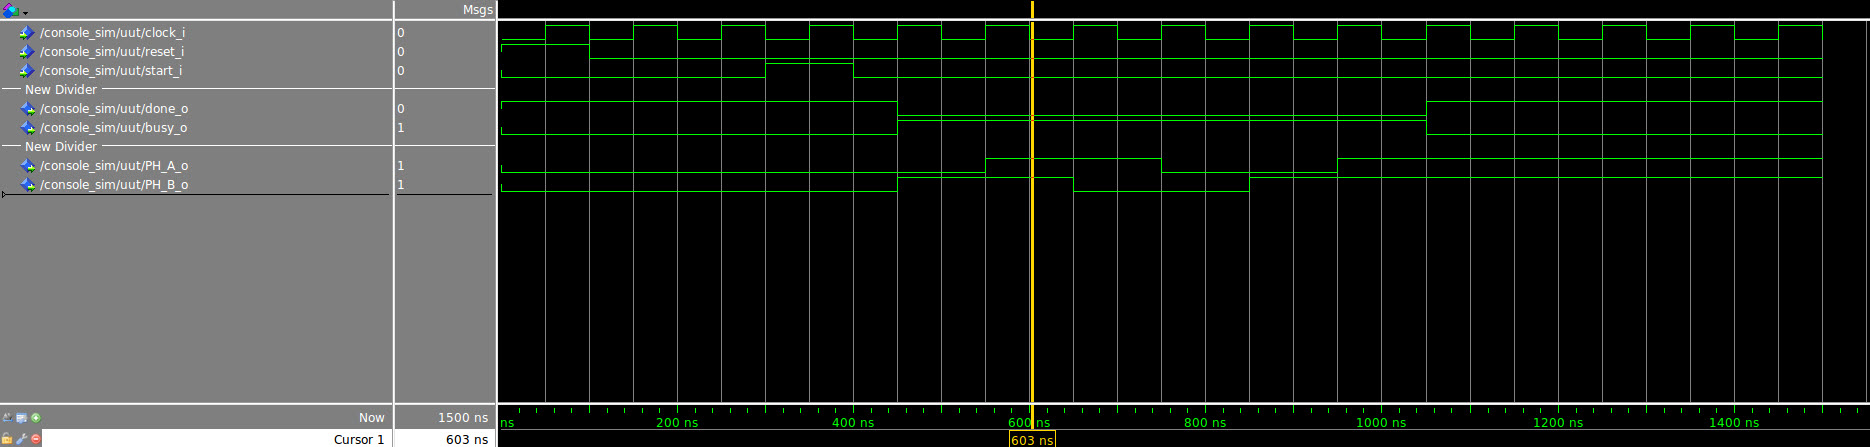
\includegraphics[angle=90,scale=0.45]{images/autoSim.jpg}\\

\end{tabular}
\newpage
\section{Synthèse}
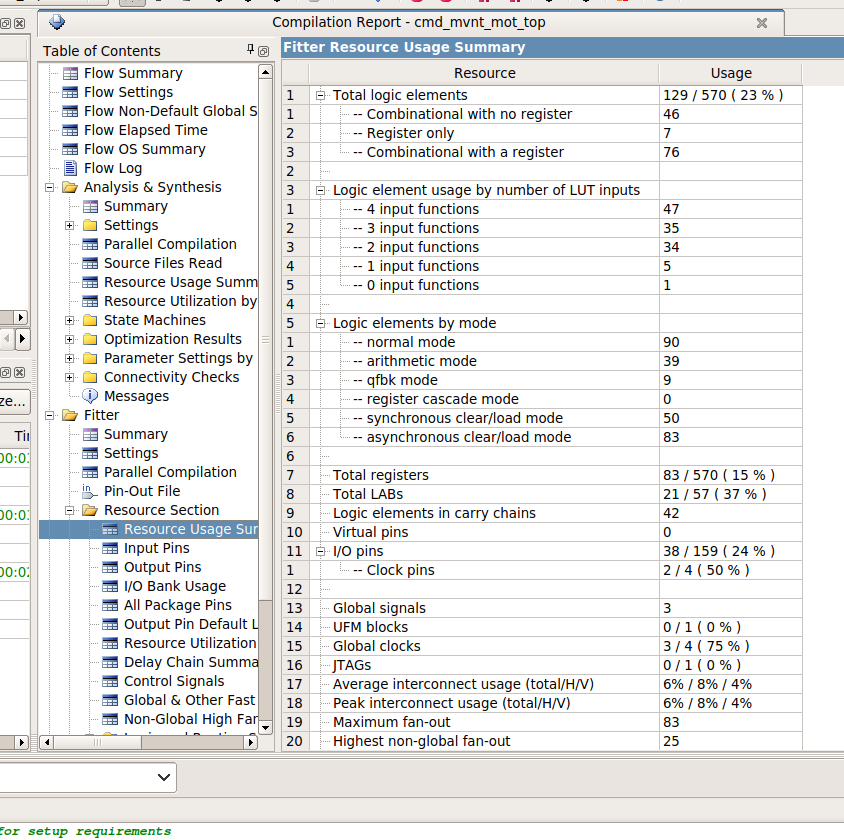
\includegraphics[scale=0.45]{images/summaryQuartus.png}\\

Lors de l'importation sur la carte, nous avons tester le fonctionnement manuel et automatique. Nous avons aussi essayer les deux direction et différentes vitesses.

\newpage
\section{VHDL}

\end{document}
